\subsubsection{Parallelization of the k-d tree build} % (fold)
\label{ssub:parallelization_of_the_k_d_tree_build}

Continuing our quest for a fast kNN search, a parallelization of the k-d tree build was introduced with RQ~\ref{rq:parallel_build}, in Section~\ref{sec:development_of_a_parallel_k_d_tree_build_algorithm}.

\textbf{RQ~\ref{rq:parallel_build}.} \emph{It is possible to parallelize the k-d tree build algorithm, in such a way that it gives a significant speed improvement compared to the serial algorithm.}

The resource question is based around the complex nature of the k-d tree build, and the uncertainty of a acceptable parallel speedup. This question was investigated though implementation prototypes, together with a thorough discussion about the parallelization and the intermediate results. 

\begin{figure}[ht!]
    \centering
    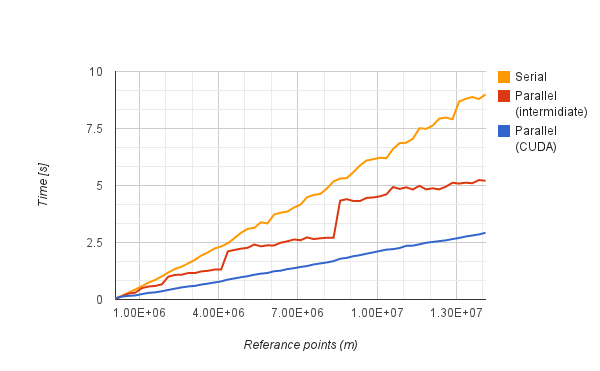
\includegraphics[width=120mm]{../gfx/final_tree_build.png}
    \caption{Comparison between serial and parallel k-d tree build performance.}
    \label{fig:final_tree_build}
\end{figure}

Figure~\ref{fig:final_tree_build} tries to answer RQ~\ref{rq:parallel_build}, by comparing the serial and parallel k-d tree build implementation. Both graphs follows the same trend, which correlates with the shared time complexity of \BigO{m\ log(m)}. We see that the impact of the parallel overhead is decreasing as the problem size increase, as the profit of multiple cores is getting more and more be dominant. Resulting in a faster parallel implementation.

To get a better picture of the parallel improvement, it is natural to talk about parallel speedup. Figure~\ref{fig:final_tree_build_speedup} shows how the parallel speedup develops, as the problem size increase. The speedup starts below $1$, indicating that the serial version is faster, but from Figure~\ref{fig:final_tree_build} one can see that the time to build such small k-d trees is almost negligible. As the problem size increase, the trend quickly changes, until the speedup flattens out. This is a typical scenario in this kind of speedup graphs. The speedup increases as the problem size allows utilization of more and more threads, until the limit is reached, and the curve flattens out into a lower gradient. Our implementation reach this flattening at a parallel speedup of around three.      

\begin{figure}[ht!]
    \centering
    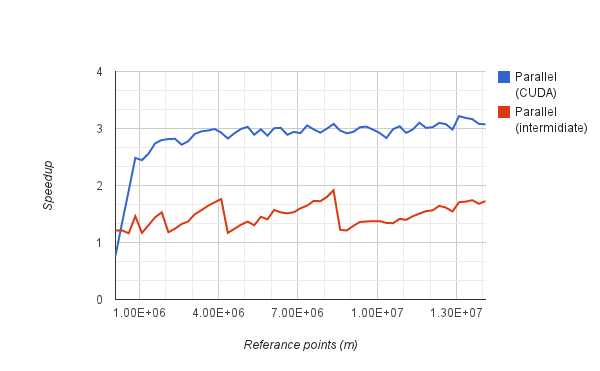
\includegraphics[width=120mm]{../gfx/final_tree_build_speedup.png}
    \caption{Parallel speedup for the k-d tree implementation for varying values of $m$.}
    \label{fig:final_tree_build_speedup}
\end{figure}

With the complex nature if a k-d tree build process, a speedup of three is acceptable, and we categorize it as a significant improvement, which answer RQ~\ref{rq:parallel_build}. 

\subsubsection{Parallelization of the All-kNN query} % (fold)
\label{ssub:parallelization_of_the_all_knn_query}

The next topic of our quest was introduced in Section~\ref{sec:development_of_a_parallel_k_d_search_algorithm}, by RQ~\ref{rq:parallel_query},

\textbf{RQ~\ref{rq:parallel_query}.} \emph{It is possible to parallelize the All-kNN query algorithm, in such a way that it gives a significant speed improvement compared to the serial algorithm.}

\begin{figure}[ht!]
    \centering
    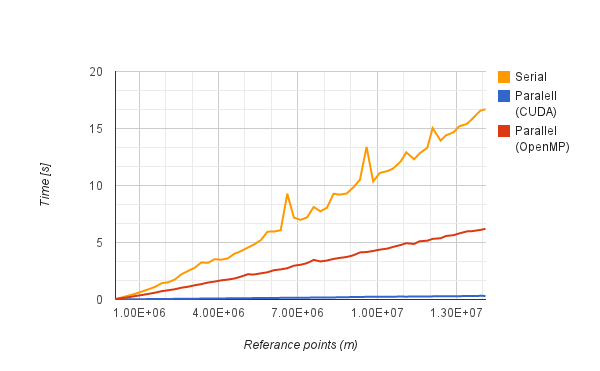
\includegraphics[width=120mm]{../gfx/final_kd_search.png}
    \caption{Comparison between serial and parallel All-kNN query performance.}
    \label{fig:final_kd_search}
\end{figure}

Figure~\ref{fig:final_kd_search} visualize the results from the two different parallel All-kNN query implementations, CUDA and OpenMP, compared to the serial version. The linear trend, also found in the k-d tree build algorithm, is not surprising, as the time complexity for all algorithms are \BigO{m\ log(m)}. Whats the parallel version improves, in terms of speed development, is the gradient. In both OpenMp and CUDA the parallel improvement is significant.

\begin{figure}[ht!]
    \centering
    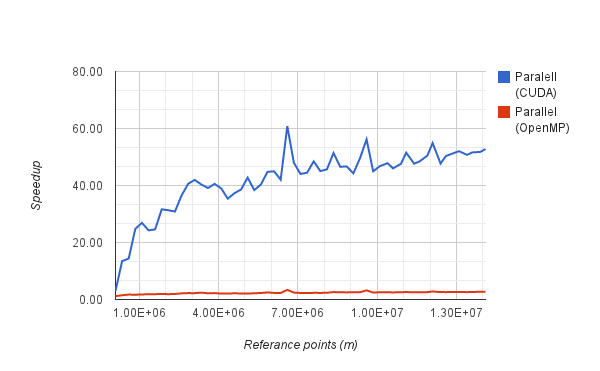
\includegraphics[width=120mm]{../gfx/final_kd_search_speedup.png}
    \caption{Parallel speedup comparison for the All-kNN query between the CUDA and OpenMP implementation.}
    \label{fig:final_kd_search_speedup}
\end{figure}

If we look at the parallel speedup, shown in Figure~\ref{fig:final_kd_search_speedup}, we can again conclude that the OpenMP version is outperformed by the CUDA implementation. Again, the trend resembles what we saw in the k-d tree build parallelization, only this time the speedup goes towards $50$ in the CUDA version. This correlations perfectly with the discussion around the parallelization strategy in Section~\ref{sub:parallelization_strategy}.      

An interesting note is that this speedup is lower then in both our and Garcia's\cite{Garcia2008} brute force implementations, which implies that speedup don't equal a fast implementations. It only implies a good parallel performance increase, compared to the serial algorithmic in use.

This conclude that our All-kNN query has a significant parallel improvement, and RQ~\ref{rq:serial-kd-tree} is answered  
% subsubsection parallelization_of_the_all_knn_query (end)
% subsubsection parallelization_of_the_k_d_tree_build (end)
